\documentclass[12pt]{article}
\usepackage{amsmath}
\usepackage{graphicx,psfrag,epsf}
\usepackage{enumerate}
\usepackage{natbib}
\usepackage{url} % not crucial - just used below for the URL 

\usepackage{amssymb, qtree, bm, multirow, textcmds, siunitx,paralist}
\usepackage{mathrsfs, float, booktabs,todonotes,amsthm, xcolor,sidenotes}
\usepackage[bb=boondox]{mathalfa}
\usepackage{tikz}
\usetikzlibrary{arrows,positioning,shapes,fit,calc}
\usepackage{amsfonts}

\pdfminorversion=4
% NOTE: To produce blinded version, replace "0" with "1" below.
\newcommand{\blind}{1}

% DON'T change margins - should be 1 inch all around.
\addtolength{\oddsidemargin}{-.5in}%
\addtolength{\evensidemargin}{-.5in}%
\addtolength{\textwidth}{1in}%
\addtolength{\textheight}{-.3in}%
\addtolength{\topmargin}{-.8in}%

\DeclareMathOperator*{\argmin}{arg\,min}
\newcolumntype{L}{>{$}l<{$}} % math-mode version of "l" column type
\def\mathbi#1{\textit{ #1}}
\def\mathB#1{\textbf{ #1}}
\def\E{\text{E}}
\def\var{\text{Var}}

\def\PQ{\begin{pmatrix}\bm{G}\\[-0.2cm]\bm{H}\end{pmatrix}}
\def\bt{\begin{pmatrix}\tilde{\bm{b}}\\[-0.2cm]\tilde{\bm{a}}\end{pmatrix}}

%\theoremstyle{theo}
\newtheorem{theo}{Theorem}[section]

\theoremstyle{definition}
\newtheorem{definition}{Definition}[section]

\theoremstyle{property}
\newtheorem{property}{Property}[section]


\begin{document}
	
	
	%\bibliographystyle{natbib}
	
	\def\spacingset#1{\renewcommand{\baselinestretch}%
		{#1}\small\normalsize} \spacingset{1}
	
	
	%%%%%%%%%%%%%%%%%%%%%%%%%%%%%%%%%%%%%%%%%%%%%%%%%%%%%%%%%%%%%%%%%%%%%%%%%%%%%%
	
	\if1\blind
	{
		\title{\bf Hierarchical Forecasts Reconciliation}
		\author{Puwasala Gamakumara\thanks{
				The authors gratefully acknowledge the support of Australian Research Council Grant DP140103220.  We also thank Professor Mervyn Silvapulle for valuable comments.}\hspace{.2cm}\\
			Department of Econometrics and Business Statistics,\\
			Monash University,\\ VIC 3800, Australia.\\
			Email: Puwasala.Gamakumara@monash.edu \\
			and \\
			Anastasios Panagiotelis\\
			Department of Econometrics and Business Statistics,\\
			Monash University,\\ VIC 3800, Australia.\\
			Email: Anastasios.Panagiotelis@monash.edu \\
			and \\
			George Athanasopoulos\\
			Department of Econometrics and Business Statistics,\\
			Monash University,\\ VIC 3800, Australia.\\
			Email: george.athanasopoulos@monash.edu \\
			and \\
			Rob J Hyndman\\
			Department of Econometrics and Business Statistics,\\
			Monash University,\\ VIC 3800, Australia.\\
			Email: rob.hyndman@monash.edu \\}
		\maketitle
	} \fi
	
	\if0\blind
	{
		\bigskip
		\bigskip
		\bigskip
		\begin{center}
			{\LARGE\bf Hierarchical Forecasts Reconciliation}
		\end{center}
		\medskip
	} \fi
	
	\bigskip
	
	
	\begin{abstract} TBC
		%  Forecast reconciliation involves adjusting forecasts to ensure coherence with aggregation constraints. We extend this concept from point forecasts to probabilistic forecasts by redefining forecast reconciliation in terms of linear functions in general, and projections more specifically. New theorems establish that the true predictive distribution can be recovered in the elliptical case by linear reconciliation, and general conditions are derived for when this is a projection. A geometric interpretation is also used to prove two new theoretical results for point forecasting; that reconciliation via projection both preserves unbiasedness and dominates unreconciled forecasts in a mean squared error sense. Strategies for forecast evaluation based on scoring rules are discussed, and it is shown that the popular log score is an improper scoring rule with respect to the class of unreconciled forecasts when the true predictive distribution coheres with aggregation constraints. Finally, evidence from a simulation study shows that reconciliation based on an oblique projection, derived from the MinT method of \citet{Wickramasuriya2017} for point forecasting, outperforms both reconciled and unreconciled alternatives.
	\end{abstract}
	
%	\noindent%
%	{\it Keywords:}  Forecast Reconciliation, Projections, Elliptical Distributions, Scoring Rules, High-dimensional Time Series.
%	\vfill
	
	\newpage
	\spacingset{1.45} % DON'T change the spacing!
	
	\section{Introduction}\label{sec:intro}
	
	
%	Large collections of time series often follow some aggregation structure. For example, the electricity demand of a country can be disaggregated according to a geographic hierarchy of states, cities, and individual households. To ensure aligned decision making, it is important that forecasts at the most disaggregated level add up to forecasts at more aggregated levels. This property is called ``coherence''.  On the other hand ``reconciliation'' is a process whereby incoherent forecasts are made coherent. Both of these concepts have been developed extensively for point forecasting. Generalising both of these concepts, particularly the latter, to probabilistic forecasting is a gap that we seek to address in this work.  We do so by first providing a novel geometric interpretation to coherence and reconciliation in the point forecasting case. This can easily be generalised to probabilistic forecasting allowing us to derive further results for elliptical distributions as well as provide insight into forecast evaluation via multivariate  scoring rules. 
%	
%	Traditional approaches to ensure coherent point forecasts produce first-stage forecasts at a single level of the hierarchy. To describe these we use the small hierarchy in Figure~\ref{fig1} where the variable labelled $Tot$ is the sum of the series $A$ and series $B$, the series $A$ is the sum of series $AA$ and series $AB$ and the series $B$ is the sum of the series $BA$ and $BB$. In the bottom-up approach \citep{Dunn1976}, forecasts are produced at the most disaggregated level (series $AA$, $AB$, $BA$ and $BB$) and then summed to recover forecasts for all higher-level series. Alternatively, in the top-down approach \citep{Gross1990}, a top-level forecast is first produced (series $Tot$) and bottom-level forecasts are recovered by disaggregating the forecast using either historical or forecasted proportions. A middle-out approach is a hybrid between these two, that for the hierarchy in Figure~\ref{fig1} would produce first stage forecasts for series $A$ and $B$.
%	
%	
%	In recent years, reconciliation methods introduced by \citet{Hyndman2011} have become increasingly popular. For these methods, first stage forecasts are independently produced for all series rather than series at a single level. Since these so-called `base' forecasts are rarely coherent in practice, they are subsequently adjusted or `reconciled' to ensure coherence.  Note that we use coherence and reconciliation as distinct terms, in contrast to their at times ambiguous usage in the past. To date, reconciliation has typically been formulated as a regression problem with alternative reconciliation methods resembling different least squares estimators. These include Ordinary Least Squares {OLS} \citep{Hyndman2011}, Weighted Least Squares {WLS} \citep{AthEtAl2017}, and a Generalised Least Squares (GLS) estimator \citep{Wickramasuriya2017} named MinT since it minimises the trace of the squared error matrix. These methods have been shown to outperform traditional alternatives across a range of simulated and real-world datasets \citep{AthEtAl2009,VanErven2015a,Wickramasuriya2017} since they use information at all levels of the hierarchy and, in some sense, hedge against the risk of model misspecification at a single level.
%	
%	A shortcoming of the existing literature is a focus on point forecasting despite an increased understanding over the past decade of the importance of providing a full predictive distribution for forecast uncertainty \citep[see][and references therein]{Gneiting2014}. Indeed to the best of our knowledge, the (as yet unpublished) work of \citep{BenTaieb2017} is the only paper to deal with coherent probabilistic forecasts, and although they reconcile the means of the predictive distributions, the overall distributions are constructed in a bottom-up fashion rather than use a reconciliation process. In contrast, the main objective of our paper is to generalise both coherence and reconciliation from point to probabilistic forecasting.
%	
%	To facilitate the extension of point forecast reconciliation to probabilistic forecasting, we first provide a geometric interpretation of existing point reconciliation methods, framing them in terms of projections. In addition to being highly intuitive, this allows us to establish a number of theoretical results. We prove two new theorems about point forecast reconciliation, the first showing that reconciliation via projections preserves the unbiasedness of base forecasts, while the second shows that reconciled forecasts dominate unreconciled forecasts via the distance reducing property of projections. We provide definitions of coherence and forecast reconciliation in the probabilistic setting, and describe how these definitions lead to a reconciliation procedure that merely involves a change of basis and marginalisation. We show that probabilistic reconciliation via linear transformations can recover the true predictive distribution as long as the latter is in the elliptical class. We provide conditions for which this linear transformation is a projection, and although this projection cannot be feasibly estimated in practice, we provide a heuristic argument in favour of MinT reconciliation.
%	
%	We also cover the topic of forecast evaluation of probabilistic forecasts via scoring rules. In particular, we prove that for a coherent data generating process, the log score is not proper with respect to incoherent forecasts. Therefore we recommend the use of the energy score or variogram score for comparing reconciled to unreconciled forecasts. Two or more reconciled forecasts can be compared using log score, energy score or variogram score, although we show that comparisons should be made on the full hierarchy for the latter two scores.
%	
%	The remainder of the paper is structured as follows. In Section~\ref{sec:definitions} coherence is defined geometrically for both point and probabilistic forecasts. Section~\ref{sec:reconciliation} contains definitions of point and probabilistic forecast reconciliation as well as our main theoretical results. In Section~\ref{sec:evaluation} we consider the evaluation of probabilistic hierarchical forecasts via scoring rules, while a simulation study comparing unreconciled probabilistic forecasts and different kinds of reconciled probabilistic forecasts is provided in Section~\ref{sec:gaussian}. Section~\ref{sec:conclusions} concludes with some discussion and thoughts on future research.
	
\section{Coherent forecasts}\label{sec:CoheForecasts}
	
	\subsection{Notation and preliminaries}\label{sec:notation}
	
    We briefly define the concept of a \emph{hierarchical time series} in a fashion similar to \cite{Wickramasuriya2017}, \cite{FPP2018} and others, before elaborating on some of the limitations of this understanding.  A \emph{hierarchical time series} is a collection of $n$ variables indexed by time, where some variables are aggregates of other variables. We let $\bm{y}_t \in \mathbb{R}^n$ be a vector comprising observations of all variables in the hierarchy at time $t$. The \emph{bottom-level series} are defined as those $m$ variables that cannot be formed as aggregates of other variables; we let $\bm{b}_t \in \mathbb{R}^m$ be a vector comprised of observations of all bottom-level series at time $t$.  The hierarchical structure of the data implies that the following holds for all $t$
    
    \begin{equation}
    \bm{y}_t = \bm{Sb}_t,
    \end{equation}
    where $\bm{S}$ is an $n \times m$ constant matrix that encodes the aggregation constraints.  
	
		\begin{figure}[H]
			\begin{center}
				\leaf{AA} \leaf{AB}
				\branch{2}{A}
				\leaf{BA} \leaf{BB}
				\branch{2}{B}
				\branch{2}{Tot}
				\qobitree
			\end{center}
			\caption{An example of a two level hierarchical structure.}\label{fig:basichier}
		\end{figure}
	
	To clarify these concepts consider the example of the hierarchy in Figure~\ref{fig:basichier}.  For this hierarchy, $n=7$, $\bm{y}_t = [y_{Tot,t},y_{A,t}, y_{B,t},y_{C,t},y_{AA,t}, y_{AB,t}, y_{BA,t}, y_{BB,t}]'$, $m=4$, $\bm{b}_t = [y_{AA,t}, y_{AB,t}, y_{BA,t}, y_{BB,t}]'$ and
	\[
	\bm{S} = \begin{pmatrix}
	1 & 1 & 1 & 1  \\
	1 & 1 & 0 & 0 \\
	0 & 0 & 1 & 1 \\
	& \multicolumn{2}{c}{\bm{I}_4} &
	\end{pmatrix},
	\]
	where $\bm{I}_4$ is the $4\times 4$ identity matrix.
	
	While such a definition is completely serviceable, it obscures the full generality of the literature on so-called hierarchical time series.  In fact, concepts such as coherence and reconciliation, defined in full below, only require the data to have two important characteristics; the first is that they are multivariate, the second is that they adhere to linear constraints.  
	
	\subsection{Coherence}\label{sec:cohpointf}
	
	The property that data adhere to some linear constraints is referred to as {\em coherence}.  We now provide definitions aimed at providing geometric intuition of hierarchical time series.
	
	 \begin{definition}[Coherent subspace]\label{def:cohspace}
	 	The $m$-dimensional linear subspace $\mathfrak{s}\subset \mathbb{R}^n$ for which a set of linear constraints holds for all $\bm{y}\in\mathfrak{s}$ is defined as the \emph{coherent subspace}.
	 \end{definition}
 
     To further illustrate, Figure \ref{fig:3D_hierarchy} depicts the most simple three variable hierarchy where $y_{Tot,t}=y_{A,t}+y_{B,t}$.  The coherent subspace is depicted as a grey $2$-dimensional plane within $3$-dimensional space, i.e. $m=2$ and $n=3$.  It is worth noting that the coherent subspace is spanned by the columns of $\bm{S}$, i.e.\ $\mathfrak{s}=\text{span}(\bm{S})$.  In Figure~\ref{fig:3D_hierarchy}, these columns are $\vec{s}_1=(1,1,0)'$ and $\vec{s}_2=(1,0,1)'$.  However, it is equally important to recognise that the hierarchy could also have been defined in terms of $y_{Tot,t}$ and $y_{A,t}$ rather than the bottom level series, $y_{A,t}$ and $y_{B,t}$. In this case the corresponding `$\bm{S}$ matrix' would have columns $(1,0,1)'$ and $(0,1,-1)'$.  However, while there are multiple ways to define an $\bm{S}$ matrix, in all cases the columns will span the same coherent subspace, which is unique.
     
     \begin{figure}[H]
     	\centering
     	\vspace{-0.9cm}
     	\small
     	\resizebox{\linewidth}{!}{
     		% Created by tikzDevice version 0.12 on 2019-05-02 18:48:27
% !TEX encoding = UTF-8 Unicode
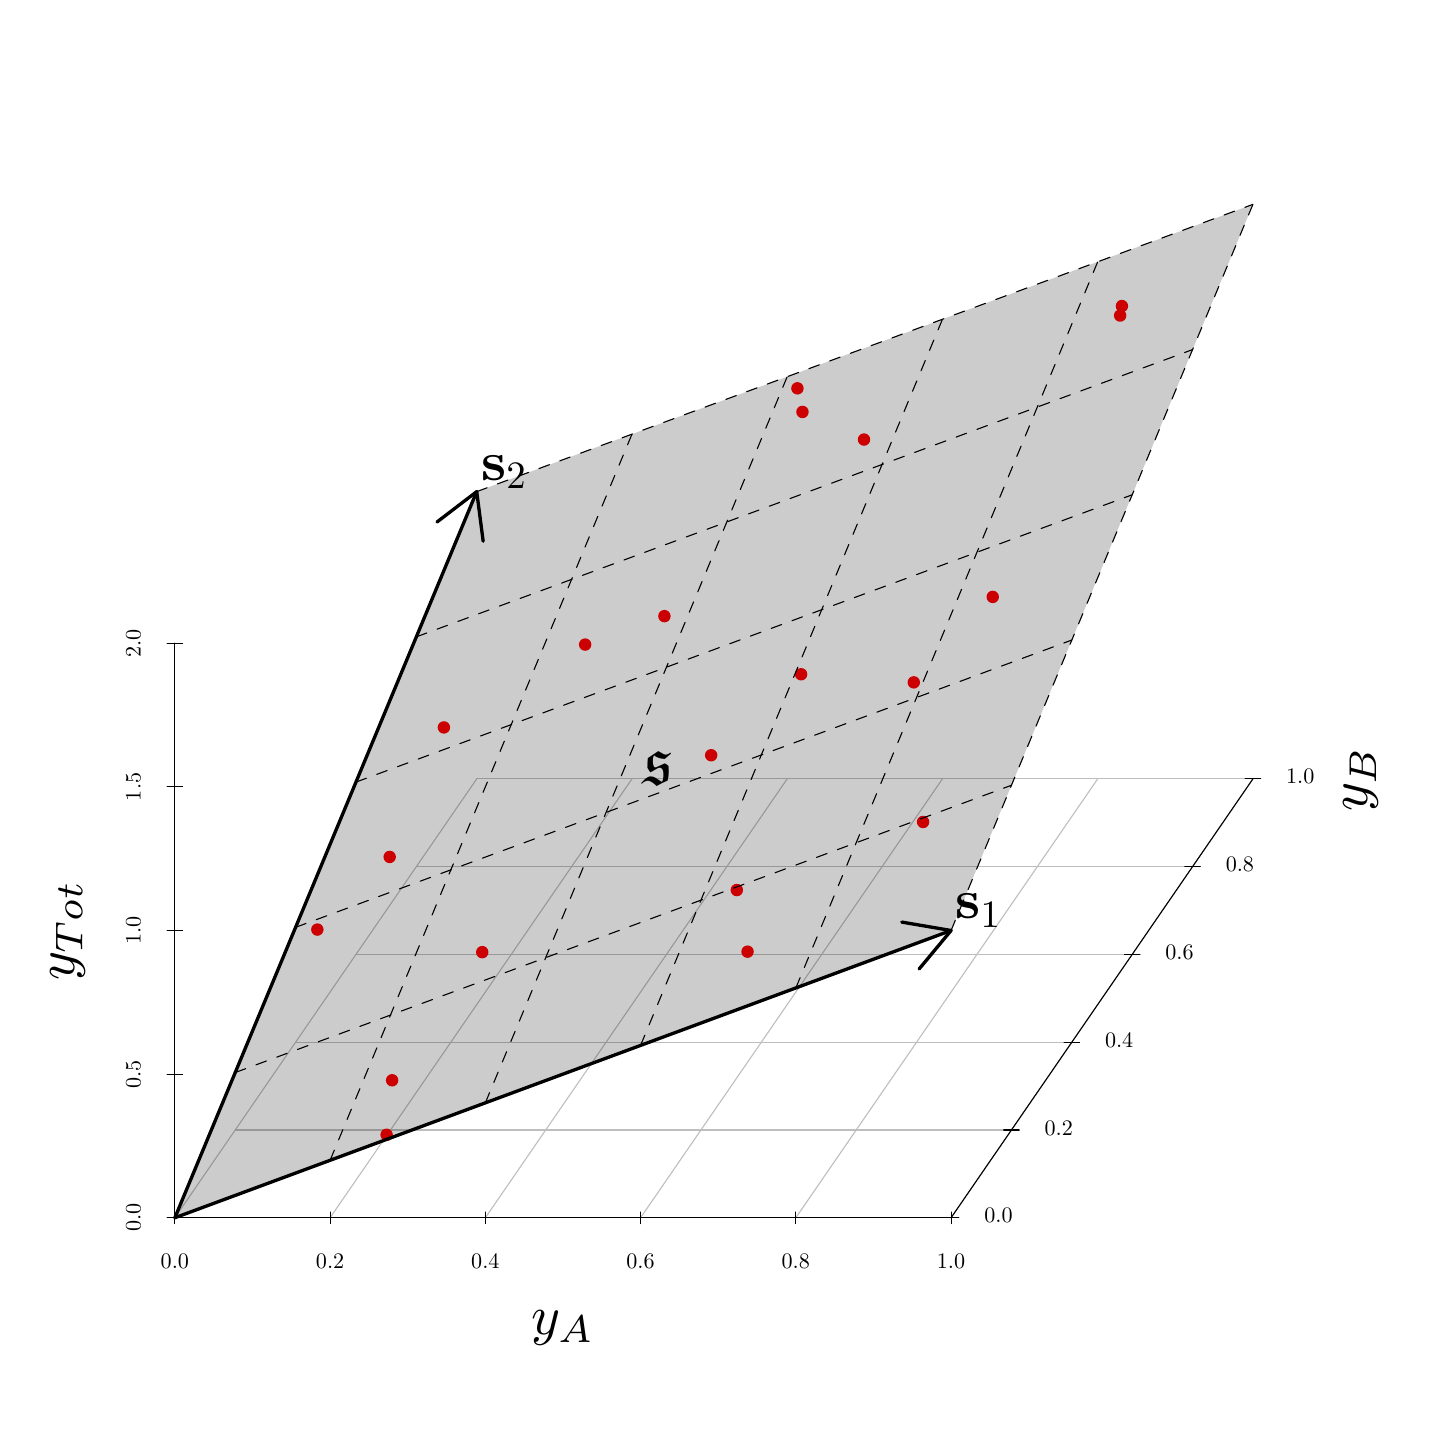
\begin{tikzpicture}[x=1pt,y=1pt]
\definecolor{fillColor}{RGB}{255,255,255}
\path[use as bounding box,fill=fillColor,fill opacity=0.00] (0,0) rectangle (505.89,505.89);
\begin{scope}
\path[clip] ( 37.20, 61.20) rectangle (468.69,456.69);
\definecolor{drawColor}{RGB}{190,190,190}

\path[draw=drawColor,line width= 0.4pt,line join=round,line cap=round] ( 53.18, 75.85) -- (162.26,234.44);

\path[draw=drawColor,line width= 0.4pt,line join=round,line cap=round] (109.28, 75.85) -- (218.36,234.44);

\path[draw=drawColor,line width= 0.4pt,line join=round,line cap=round] (165.38, 75.85) -- (274.45,234.44);

\path[draw=drawColor,line width= 0.4pt,line join=round,line cap=round] (221.47, 75.85) -- (330.55,234.44);

\path[draw=drawColor,line width= 0.4pt,line join=round,line cap=round] (277.57, 75.85) -- (386.65,234.44);

\path[draw=drawColor,line width= 0.4pt,line join=round,line cap=round] (333.67, 75.85) -- (442.74,234.44);

\path[draw=drawColor,line width= 0.4pt,line join=round,line cap=round] ( 53.18, 75.85) -- (333.67, 75.85);

\path[draw=drawColor,line width= 0.4pt,line join=round,line cap=round] ( 75.00,107.57) -- (355.48,107.57);

\path[draw=drawColor,line width= 0.4pt,line join=round,line cap=round] ( 96.81,139.28) -- (377.30,139.28);

\path[draw=drawColor,line width= 0.4pt,line join=round,line cap=round] (118.63,171.00) -- (399.11,171.00);

\path[draw=drawColor,line width= 0.4pt,line join=round,line cap=round] (140.44,202.72) -- (420.93,202.72);

\path[draw=drawColor,line width= 0.4pt,line join=round,line cap=round] (162.26,234.44) -- (442.74,234.44);
\definecolor{drawColor}{RGB}{0,0,0}

\path[draw=drawColor,line width= 0.4pt,line join=round,line cap=round] (330.86, 75.85) -- (336.47, 75.85);

\path[draw=drawColor,line width= 0.4pt,line join=round,line cap=round] (352.68,107.57) -- (358.29,107.57);

\path[draw=drawColor,line width= 0.4pt,line join=round,line cap=round] (374.49,139.28) -- (380.10,139.28);

\path[draw=drawColor,line width= 0.4pt,line join=round,line cap=round] (396.31,171.00) -- (401.92,171.00);

\path[draw=drawColor,line width= 0.4pt,line join=round,line cap=round] (418.12,202.72) -- (423.73,202.72);

\path[draw=drawColor,line width= 0.4pt,line join=round,line cap=round] (439.94,234.44) -- (445.55,234.44);

\path[draw=drawColor,line width= 0.4pt,line join=round,line cap=round] ( 53.18, 73.77) -- ( 53.18, 77.92);

\path[draw=drawColor,line width= 0.4pt,line join=round,line cap=round] (109.28, 73.77) -- (109.28, 77.92);

\path[draw=drawColor,line width= 0.4pt,line join=round,line cap=round] (165.38, 73.77) -- (165.38, 77.92);

\path[draw=drawColor,line width= 0.4pt,line join=round,line cap=round] (221.47, 73.77) -- (221.47, 77.92);

\path[draw=drawColor,line width= 0.4pt,line join=round,line cap=round] (277.57, 73.77) -- (277.57, 77.92);

\path[draw=drawColor,line width= 0.4pt,line join=round,line cap=round] (333.67, 73.77) -- (333.67, 77.92);

\path[draw=drawColor,line width= 0.4pt,line join=round,line cap=round] ( 50.38, 75.85) -- ( 55.99, 75.85);

\path[draw=drawColor,line width= 0.4pt,line join=round,line cap=round] ( 50.38,127.75) -- ( 55.99,127.75);

\path[draw=drawColor,line width= 0.4pt,line join=round,line cap=round] ( 50.38,179.65) -- ( 55.99,179.65);

\path[draw=drawColor,line width= 0.4pt,line join=round,line cap=round] ( 50.38,231.55) -- ( 55.99,231.55);

\path[draw=drawColor,line width= 0.4pt,line join=round,line cap=round] ( 50.38,283.45) -- ( 55.99,283.45);
\end{scope}
\begin{scope}
\path[clip] (  0.00,  0.00) rectangle (505.89,505.89);
\definecolor{drawColor}{RGB}{0,0,0}

\node[text=drawColor,anchor=base,inner sep=0pt, outer sep=0pt, scale=  0.80] at ( 53.18, 57.60) {0.0};

\node[text=drawColor,anchor=base,inner sep=0pt, outer sep=0pt, scale=  0.80] at (109.28, 57.60) {0.2};

\node[text=drawColor,anchor=base,inner sep=0pt, outer sep=0pt, scale=  0.80] at (165.38, 57.60) {0.4};

\node[text=drawColor,anchor=base,inner sep=0pt, outer sep=0pt, scale=  0.80] at (221.47, 57.60) {0.6};

\node[text=drawColor,anchor=base,inner sep=0pt, outer sep=0pt, scale=  0.80] at (277.57, 57.60) {0.8};

\node[text=drawColor,anchor=base,inner sep=0pt, outer sep=0pt, scale=  0.80] at (333.67, 57.60) {1.0};

\node[text=drawColor,rotate= 90.00,anchor=base,inner sep=0pt, outer sep=0pt, scale=  0.80] at ( 40.80, 75.85) {0.0};

\node[text=drawColor,rotate= 90.00,anchor=base,inner sep=0pt, outer sep=0pt, scale=  0.80] at ( 40.80,127.75) {0.5};

\node[text=drawColor,rotate= 90.00,anchor=base,inner sep=0pt, outer sep=0pt, scale=  0.80] at ( 40.80,179.65) {1.0};

\node[text=drawColor,rotate= 90.00,anchor=base,inner sep=0pt, outer sep=0pt, scale=  0.80] at ( 40.80,231.55) {1.5};

\node[text=drawColor,rotate= 90.00,anchor=base,inner sep=0pt, outer sep=0pt, scale=  0.80] at ( 40.80,283.45) {2.0};
\end{scope}
\begin{scope}
\path[clip] ( 37.20, 61.20) rectangle (468.69,456.69);
\definecolor{drawColor}{RGB}{0,0,0}

\node[text=drawColor,anchor=base west,inner sep=0pt, outer sep=0pt, scale=  0.80] at (345.67, 74.01) {0.0};

\node[text=drawColor,anchor=base west,inner sep=0pt, outer sep=0pt, scale=  0.80] at (367.48,105.73) {0.2};

\node[text=drawColor,anchor=base west,inner sep=0pt, outer sep=0pt, scale=  0.80] at (389.30,137.45) {0.4};

\node[text=drawColor,anchor=base west,inner sep=0pt, outer sep=0pt, scale=  0.80] at (411.11,169.16) {0.6};

\node[text=drawColor,anchor=base west,inner sep=0pt, outer sep=0pt, scale=  0.80] at (432.93,200.88) {0.8};

\node[text=drawColor,anchor=base west,inner sep=0pt, outer sep=0pt, scale=  0.80] at (454.74,232.60) {1.0};

\path[draw=drawColor,line width= 0.4pt,line join=round,line cap=round] ( 53.18, 75.85) --
	(333.67, 75.85);
\end{scope}
\begin{scope}
\path[clip] (  0.00,  0.00) rectangle (505.89,505.89);
\definecolor{drawColor}{RGB}{0,0,0}

\node[text=drawColor,anchor=base,inner sep=0pt, outer sep=0pt, scale=  2.00] at (193.42, 33.60) {$y_A$};
\end{scope}
\begin{scope}
\path[clip] ( 37.20, 61.20) rectangle (468.69,456.69);
\definecolor{drawColor}{RGB}{0,0,0}

\path[draw=drawColor,line width= 0.4pt,line join=round,line cap=round] (333.67, 75.85) --
	(442.74,234.44);
\end{scope}
\begin{scope}
\path[clip] (  0.00,  0.00) rectangle (505.89,505.89);
\definecolor{drawColor}{RGB}{0,0,0}

\node[text=drawColor,rotate= 90.00,anchor=base,inner sep=0pt, outer sep=0pt, scale=  2.00] at (484.29,234.44) {$y_B$};
\end{scope}
\begin{scope}
\path[clip] ( 37.20, 61.20) rectangle (468.69,456.69);
\definecolor{drawColor}{RGB}{0,0,0}

\path[draw=drawColor,line width= 0.4pt,line join=round,line cap=round] ( 53.18, 75.85) --
	( 53.18,283.45);
\end{scope}
\begin{scope}
\path[clip] (  0.00,  0.00) rectangle (505.89,505.89);
\definecolor{drawColor}{RGB}{0,0,0}

\node[text=drawColor,rotate= 90.00,anchor=base,inner sep=0pt, outer sep=0pt, scale=  2.00] at ( 16.80,179.65) {$y_{Tot}$};
\end{scope}
\begin{scope}
\path[clip] ( 37.20, 61.20) rectangle (468.69,456.69);
\definecolor{fillColor}{RGB}{255,0,0}

\path[fill=fillColor] (278.15,375.56) circle (  2.25);

\path[fill=fillColor] (279.97,367.03) circle (  2.25);

\path[fill=fillColor] (395.40,405.29) circle (  2.25);

\path[fill=fillColor] (394.76,401.87) circle (  2.25);

\path[fill=fillColor] (302.20,357.05) circle (  2.25);

\path[fill=fillColor] (201.44,282.97) circle (  2.25);

\path[fill=fillColor] (230.08,293.24) circle (  2.25);

\path[fill=fillColor] (150.40,253.03) circle (  2.25);

\path[fill=fillColor] (348.72,300.19) circle (  2.25);

\path[fill=fillColor] (279.47,272.24) circle (  2.25);

\path[fill=fillColor] (130.81,206.23) circle (  2.25);

\path[fill=fillColor] (246.98,242.98) circle (  2.25);

\path[fill=fillColor] (320.19,269.31) circle (  2.25);

\path[fill=fillColor] (104.67,179.99) circle (  2.25);

\path[fill=fillColor] (164.26,171.82) circle (  2.25);

\path[fill=fillColor] (256.24,194.27) circle (  2.25);

\path[fill=fillColor] (323.55,218.87) circle (  2.25);

\path[fill=fillColor] (131.69,125.53) circle (  2.25);

\path[fill=fillColor] (260.12,172.00) circle (  2.25);

\path[fill=fillColor] (129.70,105.84) circle (  2.25);
\definecolor{fillColor}{RGB}{0,0,0}

\path[fill=fillColor,fill opacity=0.20] ( 53.18, 75.85) --
	(162.26,338.24) --
	(442.74,442.04) --
	(333.67,179.65) --
	cycle;
\definecolor{drawColor}{RGB}{0,0,0}

\path[draw=drawColor,line width= 0.4pt,dash pattern=on 4pt off 4pt ,line join=round,line cap=round] ( 53.18, 75.85) -- (162.26,338.24);

\path[draw=drawColor,line width= 0.4pt,dash pattern=on 4pt off 4pt ,line join=round,line cap=round] (109.28, 96.61) -- (218.36,359.00);

\path[draw=drawColor,line width= 0.4pt,dash pattern=on 4pt off 4pt ,line join=round,line cap=round] (165.38,117.37) -- (274.45,379.76);

\path[draw=drawColor,line width= 0.4pt,dash pattern=on 4pt off 4pt ,line join=round,line cap=round] (221.47,138.13) -- (330.55,400.52);

\path[draw=drawColor,line width= 0.4pt,dash pattern=on 4pt off 4pt ,line join=round,line cap=round] (277.57,158.89) -- (386.65,421.28);

\path[draw=drawColor,line width= 0.4pt,dash pattern=on 4pt off 4pt ,line join=round,line cap=round] (333.67,179.65) -- (442.74,442.04);

\path[draw=drawColor,line width= 0.4pt,dash pattern=on 4pt off 4pt ,line join=round,line cap=round] ( 53.18, 75.85) -- (333.67,179.65);

\path[draw=drawColor,line width= 0.4pt,dash pattern=on 4pt off 4pt ,line join=round,line cap=round] ( 75.00,128.33) -- (355.48,232.13);

\path[draw=drawColor,line width= 0.4pt,dash pattern=on 4pt off 4pt ,line join=round,line cap=round] ( 96.81,180.80) -- (377.30,284.61);

\path[draw=drawColor,line width= 0.4pt,dash pattern=on 4pt off 4pt ,line join=round,line cap=round] (118.63,233.28) -- (399.11,337.09);

\path[draw=drawColor,line width= 0.4pt,dash pattern=on 4pt off 4pt ,line join=round,line cap=round] (140.44,285.76) -- (420.93,389.56);

\path[draw=drawColor,line width= 0.4pt,dash pattern=on 4pt off 4pt ,line join=round,line cap=round] (162.26,338.24) -- (442.74,442.04);

\path[draw=drawColor,line width= 1.2pt,line join=round,line cap=round] ( 53.18, 75.85) -- (333.67,179.65);

\path[draw=drawColor,line width= 1.2pt,line join=round,line cap=round] (322.13,165.75) --
	(333.67,179.65) --
	(315.86,182.69);

\path[draw=drawColor,line width= 1.2pt,line join=round,line cap=round] ( 53.18, 75.85) -- (162.26,338.24);

\path[draw=drawColor,line width= 1.2pt,line join=round,line cap=round] (164.59,320.32) --
	(162.26,338.24) --
	(147.91,327.26);

\node[text=drawColor,anchor=base west,inner sep=0pt, outer sep=0pt, scale=  2.00] at (335.27,183.85) {\bfseries s};

\node[text=drawColor,anchor=base west,inner sep=0pt, outer sep=0pt, scale=  1.40] at (344.34,180.84) {1};

\node[text=drawColor,anchor=base west,inner sep=0pt, outer sep=0pt, scale=  2.00] at (163.87,342.44) {\bfseries s};

\node[text=drawColor,anchor=base west,inner sep=0pt, outer sep=0pt, scale=  1.40] at (172.94,339.43) {2};

\node[text=drawColor,anchor=base west,inner sep=0pt, outer sep=0pt, scale=  1.00] at (222.57,232.24) {{\Huge $\mathfrak{s}$}};
\end{scope}
\end{tikzpicture}

     	}
     	\caption{Depiction of a three dimensional hierarchy with $y_{\text{Tot}} = y_{\text{A}} + y_{\text{B}}$. The gray colour two dimensional plane reflects the coherent subspace $\mathfrak{s}$ where $\vec{s}_1 = (1,1,0)'$ and $\vec{s}_2 = (1, 0, 1)'$ are basis vectors that spans $\mathfrak{s}$. The points in $\mathfrak{s}$ represents realisations or coherent forecasts}\label{fig:3D_hierarchy}
     \end{figure}
     
	 \begin{definition}[Hierarchical Time Series]\label{def:cohspace}
	 	A hierarchical time series is an $n$-dimensional multivariate time series such that all observed values $\bm{y}_1,\ldots,\bm{y}_T$ and all future values $\bm{y}_{T+1},\bm{y}_{T+2},\ldots$  lie in the coherent subspace, i.e. $\bm{y}_t\in\mathfrak{s}\quad\forall t$.
	 \end{definition}
	 
	 Despite the common use of the term {\em hierarchical time series}, it should be clear from the definition that the data need not necessarily follow a hierarchy.  Also notable by its absence in the above definition is any reference to {\em aggregation}. In some ways, terms such as {\em hierarchical} and {\em aggregation} can be misleading since the literature has covered instances that cannot easily be depicted in a similar fashion to Figure~\ref{fig:basichier} and or do not involve aggregation. {\bf Include brief summary of all non-traditional hierarchies - e.g. grouped hierarchies, temporal hierarchies with wierd overlapping, problems where we look at differences between variables etc.}  Finally, although the Definition~\ref{def:cohspace} makes clear reference to time series, this definition can be easily generalised to any vector-valued data for which some linear constraints are known to hold for all realisations.
	 
	 
	 
	
%	It will sometimes be useful to think of pre-multiplication by $\bm{S}$ as a mapping from $\mathbb{R}^m$ to $\mathbb{R}^n$, in which case we use the notation $s(.)$. Although the codomain of $s(.)$ is $\mathbb{R}^n$, its image is the coherent space $\mathfrak{s}$ as depicted in Figure~\ref{fig2}.
%	
%	\begin{figure}[H]
%		\begin{center}
%			\begin{tikzpicture}[
%			>=stealth,
%			bullet/.style={
%				fill=black,
%				circle,
%				minimum width=1.5cm,
%				inner sep=0pt
%			},
%			projection/.style={
%				->,
%				thick,
%				label,
%				shorten <=2pt,
%				shorten >=2pt
%			},
%			every fit/.style={
%				ellipse,
%				draw,
%				inner sep=0pt
%			}
%			]
%			\node at (2,3) {$s$};
%			\node at (0,5) {$\mathbb{R}^m$(domain of $s$)};
%			\node at (4,5) {$\mathbb{R}^n$(codomain of $s$)};
%			\node at (4.7,2.0) {$\mathfrak{s}$(image of $s$)};
%			%\node[bullet,label=below:$f(x)$] at (4,2.5){};
%			\draw (0,2.5) ellipse (1.02cm and 2.2cm);
%			\draw (4,2.5) ellipse (1.02cm and 2.2cm);
%			\draw (4,2.5) ellipse (0.51cm and 1.1cm);
%			\draw[projection, label=below:$f$] (0.3,2.5) -- (3.8,2.5) ;
%			\end{tikzpicture}
%		\end{center}
%		\caption{The domain, codomain and image of the mapping $s$.}\label{fig2}
%	\end{figure}
	
	\begin{definition}[Coherent Point Forecasts]\label{def:cohpoint}
		Let $\breve{\bm{y}}_{t+h|t} \in \mathbb{R}^n$ be a vector of point forecasts of all series in the hierarchy at time $t+h$, made using information up to and including time $t$. Then $\breve{\bm{y}}_{t+h|t}$ is \emph{coherent} if $\breve{\bm{y}}_{t+h|t} \in \mathfrak{s}$.
	\end{definition}

    Without any loss of generality, that above definition could also be applied to prediction for multivariate data in general, rather than just forecasting of time series.  While the observed data will be coherent by definition, it is important to note that there are a number of reasons why forecasts or predictions may be incoherent.  \todo{some discussion about why reconciliation v single level}    
    
    First, since applications of hierarchical forecasting tend to be very high dimensional a common strategy in practice is to produce forecasts for each time series independently using univariate models.  Second, even where a multivariate model is used for the full vector of observations, it may be difficult to capture the linear constraints inherent in the data particularly for complicated non-linear models.  Third, in some cases judgemental adjustments may be made inducing incoherent forecasts. 
	
	
	
\section{Forecast reconciliation}\label{sec:Reconciliation}
	
	As discussed in the previous section, for a number of reasons, coherence is not guaranteed when forecasts are produced for all series.  To ensure aligned decision making, it is desirable to adjust forecasts ex post to ensure coherence.  This process is referred to as {\em reconciliation}.  In the most general terms, reconciliation can be defined as follows
	
	\begin{definition}[Reconciled forecasts]\label{def:reconpoint}
		Let $\psi$ be a mapping, $\psi:\mathbb{R}^n\rightarrow\mathfrak{s}$.  The point forecast $\tilde{\bm{y}}_{t+h|t}=\psi\left(\hat{\bm{y}}_{t+h|t}\right)$ is said to ``reconcile'' $\hat{\bm{y}}_{t+h|t}$ with respect to the mapping $\psi(.)$
	\end{definition}
	
	All reconciliation methods that we are aware of consider a linear mapping for $\psi$, which involves pre-multiplying base forecasts by an $n\times n$ matrix that has $\mathfrak{s}$ as its image.  One way to achieve this is with a matrix $\bm{SG}$, where $\bm{G}$ is an $(n-m)\times n$ matrix  (with some authors using $\bm{P}$ used in place of $\bm{G}$).  This facilitates an interpretation of reconciliation as a two-step process, in the first step, base forecasts $\hat{\bm{y}}_{t+h|t}$ are combined to form a new set of bottom level forecasts, in the second step, these mapped to a full vector of coherent forecasts via pre-multiplication by $\bm{S}$.  
	
	Although pre-multiplying base forecasts by $\bm{SG}$ will result in coherent forecasts, a number of desirable properties arise when $\bm{SG}$ has the specific structure of a {\em projection} matrix onto $\mathfrak{s}$.  In general a projection matrix has the idemoptence property, i.e. $\bm{SG}^2=\bm{SG}$.  However a much more important property of projection matrices, used in multiple instances below, is that any vector lying in the image of the projection will be mapped onto itself by that projection. \todo{perhaps find a reference - it is so fundamental that is is on wikipedia and wolfram mathworld}  In our context this means that for any $\bm{v}\in\mathfrak{s}$, $\bm{SGv}=\bm{v}$.
	
	We begin by considering the special case of an orthogonal projection whereby $\bm{G}=\left(\bm{S}'\bm{S}\right)^{-1}\bm{S}'$.  This is equivalent to so called OLS reconciliation as introduced by \cite{Hyndman2011} where the connection between OLS and orthogonal projection should be clear.
	
	\subsection{Orthogonal projection}
	
	In this section we discuss two sensible properties that can be achieved by reconciliation via orthogonal projection.  The  first is that reconciliation should adjust the base forecasts as little as possible, i.e. the base and reconciled forecast should be `close'.  The second is that reconciliation in some sense should improve forecast accuracy, or more loosely, that the reconciled forecast should be `closer' to the truth.  
	
	To address the first of these properties we make the concept of closeness more concrete, by considering the Euclidean distance between the base forecast $\hat{\bm{y}}$ and the reconciled forecast  $\tilde{\bm{y}}$.  A property of an orthogonal projection is that the distance between $\hat{\bm{y}}$ and $\tilde{\bm{y}}$ will be as small as possible while still ensuring that $\tilde{\bm{y}}\in\mathfrak{s}$.  In this sense reconciliation via orthogonal projection does leads to the smallest possible adjustments of the base forecasts.
	
	The second property introduced above has been the focus of theoretical results in the forecast reconciliation literature.  He we provide a more streamlined version of proofs by \cite{VanErven2015a} and \cite{Wickramasuriya2017} before providing geometrical intuition aimed at simplifying the reader's understanding of these proofs.
	
	Consider the Euclidean distance between a forecast and the target. This is equivalent to the root of the sum of squared errors over the entire hierarchy. Let $\bm{y}_{t+h}$ be the realisation of the data generating process at time $t+h$, and let $\|\bm{v}\|_2$ be the $L_2$ norm of vector $\bm{v}$. The following theorem shows that reconciliation never increases, and in most cases reduces, the sum of squared errors of point forecasts.
	
	
	\begin{theo}[Distance reducing property]\label{th:distred}
		If $\tilde{\bm{y}}_{t+h|t}=\bm{S}\bm{G}\hat{\bm{y}}_{t+h|t}$, where $\bm{G}$ is such that $\bm{S}\bm{G}$ is an orthogonal projection onto $\mathfrak{s}$, then the following inequality holds:
		\begin{equation}
		\|(\tilde{\bm{y}}_{t+h|t}-\bm{y}_{t+h})\|^2_2\le\|(\hat{\bm{y}}_{t+h|t}-\bm{y}_{t+h})\|^2_2.
		\end{equation}
	\end{theo}
	\begin{proof}
		Since the aggregation constraints must hold for all realisations, $\bm{y}_{t+h}\in\mathfrak{s}$ and $\bm{y}_{t+h}=\bm{S}\bm{G}\bm{y}_{t+h}$ whenever $\bm{S}\bm{G}$ is a projection onto $\mathfrak{s}$. Therefore,
		\begin{align}
		\|(\tilde{\bm{y}}_{t+h|t}-\bm{y}_{t+h})\|_2&=\|(\bm{S}\bm{G}\hat{\bm{y}}_{t+h|t}-\bm{S}\bm{G}\bm{y}_{t+h})\|_2\\
		&=\|\bm{S}\bm{G}(\hat{\bm{y}}_{t+h|t}-\bm{y}_{t+h})\|_2.
		\end{align}
		The Cauchy-Schwarz inequality can be used to show that orthogonal projections are bounded operators \citep{Hun2001}, therefore
		\begin{equation*}
		\|\bm{S}\bm{G}(\hat{\bm{y}}_{t+h|t}-\bm{y}_{t+h})\|_2\le
		\|(\hat{\bm{y}}_{t+h|t}-\bm{y}_{t+h})\|_2.
		\end{equation*}
	\end{proof}
	The inequality is strict whenever $\hat{\bm{y}}_{t+h|t}\notin\mathfrak{s}$.
	
	\todo{compare to van Erven and Wickremasuriya more explictly}
	
	The simple geometric intuition behind the proof is demonstrated in Figure~\ref{fig:Schematic_OLSRecon}.  In this schematic, the coherent subspace is depicted as a black arrow.  The base forecast $\hat{\bm{y}}$ is shown as a blue dot.  Since it is incoherent it does not lie in $\mathfrak{s}$.  Reconciliation is an orthogonal projection from $\hat{\bm{y}}$ to the coherent subspace yielding the reconciled forecast $\tilde{\bm{y}}$ shown in red.  Finally, the target of the forecast $\bm{y}$ is displayed as a black point, and although its exact location is unknown to the forecaster, it is known that it will lie somewhere along the coherent subspace.
	
	\begin{figure}[H]
		\centering
		\vspace{-0.9cm}
		\tiny
		\resizebox{\linewidth}{!}{% Created by tikzDevice version 0.12 on 2019-08-21 19:50:39
% !TEX encoding = UTF-8 Unicode
\begin{tikzpicture}[x=1pt,y=1pt]
\definecolor{fillColor}{RGB}{255,255,255}
\path[use as bounding box,fill=fillColor,fill opacity=0.00] (0,0) rectangle (289.08,289.08);
\begin{scope}
\path[clip] ( 49.20, 61.20) rectangle (263.88,239.88);
\definecolor{drawColor}{RGB}{0,0,0}

\path[draw=drawColor,line width= 0.4pt,line join=round,line cap=round] ( 87.60, 49.44) --
	( 87.60,196.50);

\path[draw=drawColor,line width= 0.4pt,line join=round,line cap=round] ( 50.84, 86.20) --
	(197.90, 86.20);

\path[draw=drawColor,line width= 1.2pt,line join=round,line cap=round] ( 87.60, 86.20) -- (216.28,150.54);

\path[draw=drawColor,line width= 1.2pt,line join=round,line cap=round] (206.33,135.46) --
	(216.28,150.54) --
	(198.25,151.62);

\node[text=drawColor,anchor=base west,inner sep=0pt, outer sep=0pt, scale=  1.00] at (222.28,148.24) {{\large $\mathfrak{s}$}};
\definecolor{drawColor}{RGB}{0,0,255}
\definecolor{fillColor}{RGB}{0,0,255}

\path[draw=drawColor,line width= 0.4pt,line join=round,line cap=round,fill=fillColor] (142.75,196.50) circle (  3.00);
\definecolor{drawColor}{RGB}{0,0,0}

\node[text=drawColor,anchor=base,inner sep=0pt, outer sep=0pt, scale=  1.00] at (142.75,214.50) {{\large $\color{blue}{\hat{\bm{y}}}$}};
\definecolor{drawColor}{RGB}{255,0,0}
\definecolor{fillColor}{RGB}{255,0,0}

\path[draw=drawColor,line width= 0.4pt,line join=round,line cap=round,fill=fillColor] (175.84,130.32) circle (  3.00);
\definecolor{drawColor}{RGB}{0,0,0}

\node[text=drawColor,anchor=base,inner sep=0pt, outer sep=0pt, scale=  1.00] at (175.84,106.58) {{\large $\color{red}{\tilde{\bm{y}}}$}};
\definecolor{drawColor}{RGB}{0,0,255}

\path[draw=drawColor,line width= 0.4pt,line join=round,line cap=round] (142.75,196.50) -- (175.84,130.32);

\path[draw=drawColor,line width= 0.4pt,line join=round,line cap=round] (160.76,140.27) --
	(175.84,130.32) --
	(176.92,148.35);
\definecolor{drawColor}{RGB}{0,0,0}

\path[draw=drawColor,line width= 0.4pt,dash pattern=on 4pt off 4pt ,line join=round,line cap=round] (142.75,196.50) -- (119.12,101.96);
\definecolor{fillColor}{RGB}{0,0,0}

\path[draw=drawColor,line width= 0.4pt,line join=round,line cap=round,fill=fillColor] (119.12,101.96) circle (  3.00);

\node[text=drawColor,anchor=base,inner sep=0pt, outer sep=0pt, scale=  1.00] at (119.12, 78.22) {{\large $\color{black}{{\bm{y}}}$}};
\end{scope}
\end{tikzpicture}
}
		\label{fig:Schematic_OLSRecon}
		\caption{$\hat{\bm{y}}$ is orthogonally projected onto $\mathfrak{s}$}
		
	\end{figure}
	
	
	Figure~\ref{fig:Schematic_OLSRecon} clearly shows that $\hat{\bm{y}}$, $\tilde{\bm{y}}$ and $\bm{y}$ form a right angled triangle.  In this triangle the distance between $\bm{y}$ and $\hat{\bm{y}}$ is the hypotenuse and therefore must be longer than the distance between $\bm{y}$ and $\tilde{\bm{y}}$.  As such reconciliation is guaranteed to reduce the squared error of the forecast.  
	
    Theorem~\ref{th:distred} is in some ways more powerful than perhaps previously understood.  It is often stated in terms of expectations\todo{check other proofs}.  However, the distance reducing property result is even stronger since it will hold for any realisation and any forecast.  Nothing needs to be assumed about the statistical properties of the data generating process or the process by which forecasts are made.  
    
    However, in other ways, Theorem~\ref{th:distred} is weaker than perhaps often understood. First, when improvements in forecast accuracy are discussed in the context of the theorem, this refers to a very specific measure of forecast accuracy.  In particular, this measure is the root of the sum of squared errors of {\em all} variables in the hierarchy.  As such, while forecast improvement is guaranteed for the hierarchy overall, reconciliation can lead to worse forecasts for individual series. Second, although orthogonal projections are guaranteed to improve on base forecasts both for all realisations and in expectation, they are not necessarily the projection that leads to the greatest improvement in forecast accuracy.  As such referring to reconciliation via orthogonal projections as `optimal' is somewhat misleading since it does not have the optimality properties of some oblique projections, in particular MinT. It is to oblique projections that we now turn our attention.
    	
	\subsection{Oblique Projections}
	
	In particular, this measure is the 
	
	One justification for using an orthogonal projection is that it leads to improved forecast accuracy in terms of the root of the sum of squared errors of {\em all} variables in the hierarchy.  A clear shortcoming of this measure of forecast accuracy is that forecasts errors in all series should not necessarily be treated equally.  For example, in hierarchies, top-level series tend to have a much larger scale than bottom level series.  Even when two series are on a similar scale, series that are more predictable or less variable will tend to be downweighted by simply aggregating square errors.  An even more sophisticated understanding may take the correlation between series into account.  All of these considerations lead towards reconciliation of the form $\tilde{\bm{y}}=\bm{S}\left(\bm{S}'\bm{W}^{-1}\bm{S}\right)^{-1}\bm{S}'\bm{W}^{-1}\hat{\bm{y}}$, where $\bm{W}$ is a symmetric matrix.  Generally, it is assumed that $\bm{W}$ is invertible, otherwise a pseudo inverse can be used.
	
	It should be noted that  $\bm{S}\left(\bm{S}'\bm{W}^{-1}\bm{S}\right)^{-1}\bm{S}'\bm{W}^{-1}$ is an oblique, rather than an orthogonal projection matrix.  However this matrix can be considered to be an orthogonal projection for a different geometry, namely the generalised Euclidean geometry with respect to $\bm{W}^{-1}$.  One way to understand this geometry is that it is the same as Euclidean geometry when all vectors are first transformed by pre-multiplying by $\bm{W}^{-1/2}$.  This leads to a transformed $\bm{S}$ matrix $\bm{S}^*=\bm{W}^{-1/2}\bm{S}$ and transformed $\hat{\bm{y}}$ and $\tilde{\bm{y}}$ vectors $\hat{\bm{y}}^*=\bm{W}^{-1/2}\hat{\bm{y}}$ and $\tilde{\bm{y}}^*=\bm{W}^{-1/2}\tilde{\bm{y}}$.  The transformed reconciled forecast results from an orthogonal projection in the transformed space since 
	
	\begin{align}
	\tilde{\bm{y}}^*&=\bm{W}^{-1/2}\tilde{\bm{y}}\\&=\bm{W}^{-1/2}\bm{S}\left(\bm{S}'\bm{W}^{-1}\bm{S}\right)^{-1}\bm{S}'\bm{W}^{-1}\hat{\bm{y}}
	\\&=\bm{S}^*\left(\bm{S}^{*'}\bm{S}^*\right)^{-1}\bm{S}^{*'}\hat{\bm{y}^*}
	\end{align}
	
	Another way of understanding the generalised Euclidean geometry is that it is defined by the norm $\bm{v}'\bm{W}^{1}\bm{v}$.  This interpretation is quite instructive when it comes to thinking about the connection between distances and loss functions.  In the generalised Euclidean geometry, the distance between the reconciled forecast and the realisation is given by $(\hat{\bm{y}}-\bm{y})'\bm{W}^{-1}(\hat{\bm{y}}-\bm{y})$.  For diagonal $\bm{W}$ this is equivalent to a weighted sum of squared error loss function and when $\bm{W}$ is a covariance matrix this is equivalent to a Mahalanobis distance.  As such Theorem~\ref{th:distred} can easily be generalised.  If the objective function is some weighted sum of squared errors, or a Mahalanobis distance, then the projection matrix $\bm{S}\left(\bm{S}'\bm{W}^{-1}\bm{S}\right)^{-1}\bm{S}'\bm{W}^{-1}$ is guaranteed to improve forecast accuracy over base forecasts, for an appropriately selected $\bm{W}$.
	
	First, the linear subspace onto which all points are projected, or the image of the projection, must be defined. In our context this can be defined by the $m$ columns of the matrix $\bm{S}$.  Second, the direction along which points are projected must be defined.  This will be achieved by defining a matrix $\bm{R}$ with $n-m$ columns then span the direction of projection. A schematic of this is presented \todo{include}.   A projection matrix can then be constructed as $\bm{S}({\bm{R}'_{\perp}}\bm{S})^{-1}\bm{R}_{\perp}'$ where, ${\bm{R}_{\perp}}$ is an $n\times m$ orthogonal complement to $\bm{R}$ such that ${\bm{R}'_{\perp}}\bm{R}=\bm{0}$. It is simple to verify that this construction satisfies the properties of a projection matrix, namely symmetry and idempotence.
	
	A straightforward choice of $\bm{R}$ for the most simple three variable hierarchy where $y_{1,t}=y_{2,t}+y_{3,t}$, is the vector $(1,-1,-1)$ which is orthogonal (in the Euclidean sense) to the columns of $\bm{S}$. In this case, the matrix $\bm{R}$ can be interpreted as a `restrictions' matrix since it has the property that $\bm{R}'\bm{y}=\bm{0}$ for coherent $\bm{y}$. In OLS reconciliation, $\bm{R}_{\perp}'= \bm{S}'$ whereas in MinT or WLS reconciliation $\bm{R}_{\perp}'$ takes the form $\bm{S'W}^{-1}$. We will be discussing these projections distinctly in the next subsection\todo{needs work}. 
	
	
	In MinT reconciliation, $\bm{R}'_\perp$ is taking the form $\bm{S}'{\bm{W}}^{-1}$, where it can be thought of as orthogonal projections after pre-multiplying by ${\bm{W}^{-1/2}}$. That is, the coordinates of incoherent space will be scaled by $\bm{W}^{-1/2}$ which is then followed by the orthogonal projection. Alternatively this can be interpreted as an oblique projections in Euclidean space where the columns of $\bm{R}$ is the `direction' along which incoherent point forecasts are projected onto the coherent space $\mathfrak{s}$ as depicted in Figure \ref{fig:pointfr_sch}. In terms of distances, MinT minimises the Euclidean distance between $\hat{\bm{y}}_{t+h|t}$ and $\tilde{\bm{y}}_{t+h|t}$ in the transformed space which is same as the scaled Euclidean distance in the original space. Latter is also referred to as the Mahalonobis distance. We also note that the WLS is a special case of MinT where $\bm{W}^{-1}$ is a diagonal matrix. 
	
	\citet{Wickramasuriya2017} showed that the MinT is optimal with respect to the mean squared forecast errors. 
	We can provide a more general geometrical explanation to this optimality using the schematic in Figure \ref{fig:MinT_justification}. Consider the h-step ahead reconciled forecast errors. These can be always approximated by the insample h-step ahead forecast errors. Since these errors are coherent, they lies in a direction that is closer to the coherent subspace $\mathfrak{s}$. Therefore if you project $\hat{\bm{y}}$ along the direction of these in-sample forecast errors, then you can get closer to the true value $\bm{y}$ as depicted in the schematic. Further, unlike OLS, the squared error for MinT reconciled forecasts is not always less than that of base forecasts in every single replication although it outperforms on average.
	
	
	
	\begin{figure}[H]
		\centering
		%\vspace{-0.9cm}
		\small
		\resizebox{\linewidth}{!}{
			% Created by tikzDevice version 0.12 on 2019-04-26 17:05:14
% !TEX encoding = UTF-8 Unicode
\begin{tikzpicture}[x=1pt,y=1pt]
\definecolor{fillColor}{RGB}{255,255,255}
\path[use as bounding box,fill=fillColor,fill opacity=0.00] (0,0) rectangle (505.89,361.35);
\begin{scope}
\path[clip] ( 49.20, 61.20) rectangle (480.69,312.15);
\definecolor{drawColor}{RGB}{0,0,0}

\path[draw=drawColor,line width= 0.4pt,line join=round,line cap=round] ( 88.68, 49.37) --
	( 88.68,302.86);

\path[draw=drawColor,line width= 0.4pt,line join=round,line cap=round] (  0.00, 91.62) --
	(505.89, 91.62);

\path[draw=drawColor,line width= 1.2pt,line join=round,line cap=round] ( 88.68, 91.62) -- (417.71,165.55);

\path[draw=drawColor,line width= 1.2pt,line join=round,line cap=round] (404.42,153.31) --
	(417.71,165.55) --
	(400.46,170.93);

\node[text=drawColor,anchor=base west,inner sep=0pt, outer sep=0pt, scale=  1.00] at (423.71,163.26) {{\huge $\mathfrak{s}$}};
\definecolor{drawColor}{RGB}{255,165,0}
\definecolor{fillColor}{RGB}{255,165,0}

\path[draw=drawColor,line width= 0.4pt,line join=round,line cap=round,fill=fillColor] ( 94.18, 99.01) circle (  2.25);

\path[draw=drawColor,line width= 0.4pt,line join=round,line cap=round,fill=fillColor] ( 22.11, 23.37) circle (  2.25);

\path[draw=drawColor,line width= 0.4pt,line join=round,line cap=round,fill=fillColor] ( 66.82, 25.86) circle (  2.25);

\path[draw=drawColor,line width= 0.4pt,line join=round,line cap=round,fill=fillColor] (182.52,249.25) circle (  2.25);

\path[draw=drawColor,line width= 0.4pt,line join=round,line cap=round,fill=fillColor] ( 88.40, 74.04) circle (  2.25);

\path[draw=drawColor,line width= 0.4pt,line join=round,line cap=round,fill=fillColor] (114.90,154.84) circle (  2.25);

\path[draw=drawColor,line width= 0.4pt,line join=round,line cap=round,fill=fillColor] ( 89.06, 96.11) circle (  2.25);

\path[draw=drawColor,line width= 0.4pt,line join=round,line cap=round,fill=fillColor] (122.85,140.22) circle (  2.25);

\path[draw=drawColor,line width= 0.4pt,line join=round,line cap=round,fill=fillColor] (106.71,114.73) circle (  2.25);

\path[draw=drawColor,line width= 0.4pt,line join=round,line cap=round,fill=fillColor] ( 88.38, 48.60) circle (  2.25);

\path[draw=drawColor,line width= 0.4pt,line join=round,line cap=round,fill=fillColor] ( 90.09,128.33) circle (  2.25);

\path[draw=drawColor,line width= 0.4pt,line join=round,line cap=round,fill=fillColor] (121.36,155.11) circle (  2.25);

\path[draw=drawColor,line width= 0.4pt,line join=round,line cap=round,fill=fillColor] ( 39.03, 12.00) circle (  2.25);

\path[draw=drawColor,line width= 0.4pt,line join=round,line cap=round,fill=fillColor] ( 66.88, 38.58) circle (  2.25);

\path[draw=drawColor,line width= 0.4pt,line join=round,line cap=round,fill=fillColor] ( 56.17, 28.22) circle (  2.25);

\path[draw=drawColor,line width= 0.4pt,line join=round,line cap=round,fill=fillColor] ( 85.80, 54.39) circle (  2.25);

\path[draw=drawColor,line width= 0.4pt,line join=round,line cap=round,fill=fillColor] ( 47.41, 52.57) circle (  2.25);

\path[draw=drawColor,line width= 0.4pt,line join=round,line cap=round,fill=fillColor] (108.94,150.09) circle (  2.25);

\path[draw=drawColor,line width= 0.4pt,line join=round,line cap=round,fill=fillColor] (136.18,139.49) circle (  2.25);

\path[draw=drawColor,line width= 0.4pt,line join=round,line cap=round,fill=fillColor] ( 95.80,121.03) circle (  2.25);

\path[draw=drawColor,line width= 0.4pt,line join=round,line cap=round,fill=fillColor] (133.02,211.06) circle (  2.25);

\path[draw=drawColor,line width= 0.4pt,line join=round,line cap=round,fill=fillColor] (131.25,206.71) circle (  2.25);

\path[draw=drawColor,line width= 0.4pt,line join=round,line cap=round,fill=fillColor] ( 82.62, 84.61) circle (  2.25);

\path[draw=drawColor,line width= 0.4pt,line join=round,line cap=round,fill=fillColor] ( 83.48, 92.54) circle (  2.25);

\path[draw=drawColor,line width= 0.4pt,line join=round,line cap=round,fill=fillColor] ( 83.01, 75.74) circle (  2.25);

\path[draw=drawColor,line width= 0.4pt,line join=round,line cap=round,fill=fillColor] ( 82.07,126.99) circle (  2.25);

\path[draw=drawColor,line width= 0.4pt,line join=round,line cap=round,fill=fillColor] ( 49.87, 16.92) circle (  2.25);

\path[draw=drawColor,line width= 0.4pt,line join=round,line cap=round,fill=fillColor] (142.07,128.38) circle (  2.25);

\path[draw=drawColor,line width= 0.4pt,line join=round,line cap=round,fill=fillColor] ( 80.59, 56.48) circle (  2.25);

\path[draw=drawColor,line width= 0.4pt,line join=round,line cap=round,fill=fillColor] ( 92.03, 84.45) circle (  2.25);

\path[draw=drawColor,line width= 0.4pt,line join=round,line cap=round,fill=fillColor] ( 34.77, 47.51) circle (  2.25);

\path[draw=drawColor,line width= 0.4pt,line join=round,line cap=round,fill=fillColor] ( 82.02,102.38) circle (  2.25);

\path[draw=drawColor,line width= 0.4pt,line join=round,line cap=round,fill=fillColor] ( 81.91, 57.67) circle (  2.25);

\path[draw=drawColor,line width= 0.4pt,line join=round,line cap=round,fill=fillColor] ( 91.54, 30.45) circle (  2.25);

\path[draw=drawColor,line width= 0.4pt,line join=round,line cap=round,fill=fillColor] ( 85.09, 91.58) circle (  2.25);

\path[draw=drawColor,line width= 0.4pt,line join=round,line cap=round,fill=fillColor] (114.07,147.15) circle (  2.25);

\path[draw=drawColor,line width= 0.4pt,line join=round,line cap=round,fill=fillColor] ( 23.54,  9.88) circle (  2.25);

\path[draw=drawColor,line width= 0.4pt,line join=round,line cap=round,fill=fillColor] (124.37,199.40) circle (  2.25);

\path[draw=drawColor,line width= 0.4pt,line join=round,line cap=round,fill=fillColor] (112.50, 94.78) circle (  2.25);

\path[draw=drawColor,line width= 0.4pt,line join=round,line cap=round,fill=fillColor] ( 64.66,114.03) circle (  2.25);

\path[draw=drawColor,line width= 0.4pt,line join=round,line cap=round,fill=fillColor] (102.23, 94.01) circle (  2.25);

\path[draw=drawColor,line width= 0.4pt,line join=round,line cap=round,fill=fillColor] ( 64.90, 41.66) circle (  2.25);

\path[draw=drawColor,line width= 0.4pt,line join=round,line cap=round,fill=fillColor] (104.00, 88.67) circle (  2.25);

\path[draw=drawColor,line width= 0.4pt,line join=round,line cap=round,fill=fillColor] ( 76.55, 93.82) circle (  2.25);

\path[draw=drawColor,line width= 0.4pt,line join=round,line cap=round,fill=fillColor] (114.00,145.02) circle (  2.25);

\path[draw=drawColor,line width= 0.4pt,line join=round,line cap=round,fill=fillColor] ( 91.12, 53.62) circle (  2.25);

\path[draw=drawColor,line width= 0.4pt,line join=round,line cap=round,fill=fillColor] (132.25,181.94) circle (  2.25);

\path[draw=drawColor,line width= 0.4pt,line join=round,line cap=round,fill=fillColor] ( 99.97,115.95) circle (  2.25);

\path[draw=drawColor,line width= 0.4pt,line join=round,line cap=round,fill=fillColor] (112.02, 85.51) circle (  2.25);

\path[draw=drawColor,line width= 0.4pt,line join=round,line cap=round,fill=fillColor] ( 71.46, 60.94) circle (  2.25);

\path[draw=drawColor,line width= 0.4pt,line join=round,line cap=round,fill=fillColor] ( 90.88, 71.97) circle (  2.25);

\path[draw=drawColor,line width= 0.4pt,line join=round,line cap=round,fill=fillColor] ( 60.68, 58.10) circle (  2.25);

\path[draw=drawColor,line width= 0.4pt,line join=round,line cap=round,fill=fillColor] (114.50,168.18) circle (  2.25);

\path[draw=drawColor,line width= 0.4pt,line join=round,line cap=round,fill=fillColor] ( 76.49, 80.62) circle (  2.25);

\path[draw=drawColor,line width= 0.4pt,line join=round,line cap=round,fill=fillColor] ( 96.16,172.67) circle (  2.25);

\path[draw=drawColor,line width= 0.4pt,line join=round,line cap=round,fill=fillColor] ( 93.92,105.11) circle (  2.25);

\path[draw=drawColor,line width= 0.4pt,line join=round,line cap=round,fill=fillColor] ( 66.24, 44.87) circle (  2.25);

\path[draw=drawColor,line width= 0.4pt,line join=round,line cap=round,fill=fillColor] ( 32.17,  1.94) circle (  2.25);

\path[draw=drawColor,line width= 0.4pt,line join=round,line cap=round,fill=fillColor] (137.25,161.64) circle (  2.25);

\path[draw=drawColor,line width= 0.4pt,line join=round,line cap=round,fill=fillColor] ( 99.50, 60.77) circle (  2.25);

\path[draw=drawColor,line width= 0.4pt,line join=round,line cap=round,fill=fillColor] (121.90,148.95) circle (  2.25);

\path[draw=drawColor,line width= 0.4pt,line join=round,line cap=round,fill=fillColor] ( 39.03, 35.67) circle (  2.25);

\path[draw=drawColor,line width= 0.4pt,line join=round,line cap=round,fill=fillColor] ( 82.94, 53.66) circle (  2.25);

\path[draw=drawColor,line width= 0.4pt,line join=round,line cap=round,fill=fillColor] ( 65.97, 56.80) circle (  2.25);

\path[draw=drawColor,line width= 0.4pt,line join=round,line cap=round,fill=fillColor] (115.19,117.23) circle (  2.25);

\path[draw=drawColor,line width= 0.4pt,line join=round,line cap=round,fill=fillColor] (100.71,123.31) circle (  2.25);

\path[draw=drawColor,line width= 0.4pt,line join=round,line cap=round,fill=fillColor] (126.96,185.26) circle (  2.25);

\path[draw=drawColor,line width= 0.4pt,line join=round,line cap=round,fill=fillColor] ( 64.06, 72.75) circle (  2.25);

\path[draw=drawColor,line width= 0.4pt,line join=round,line cap=round,fill=fillColor] (141.63,165.15) circle (  2.25);

\path[draw=drawColor,line width= 0.4pt,line join=round,line cap=round,fill=fillColor] (138.45,121.76) circle (  2.25);

\path[draw=drawColor,line width= 0.4pt,line join=round,line cap=round,fill=fillColor] (119.03,142.68) circle (  2.25);

\path[draw=drawColor,line width= 0.4pt,line join=round,line cap=round,fill=fillColor] ( 86.52, 93.23) circle (  2.25);

\path[draw=drawColor,line width= 0.4pt,line join=round,line cap=round,fill=fillColor] (104.60,129.84) circle (  2.25);

\path[draw=drawColor,line width= 0.4pt,line join=round,line cap=round,fill=fillColor] ( 79.80, 90.71) circle (  2.25);

\path[draw=drawColor,line width= 0.4pt,line join=round,line cap=round,fill=fillColor] ( 87.05,115.16) circle (  2.25);

\path[draw=drawColor,line width= 0.4pt,line join=round,line cap=round,fill=fillColor] ( 84.75,111.90) circle (  2.25);

\path[draw=drawColor,line width= 0.4pt,line join=round,line cap=round,fill=fillColor] (108.43,143.36) circle (  2.25);

\path[draw=drawColor,line width= 0.4pt,line join=round,line cap=round,fill=fillColor] ( 80.42,105.59) circle (  2.25);

\path[draw=drawColor,line width= 0.4pt,line join=round,line cap=round,fill=fillColor] ( 80.86, 68.23) circle (  2.25);

\path[draw=drawColor,line width= 0.4pt,line join=round,line cap=round,fill=fillColor] ( 57.01, 71.38) circle (  2.25);

\path[draw=drawColor,line width= 0.4pt,line join=round,line cap=round,fill=fillColor] ( 65.41, 48.29) circle (  2.25);

\path[draw=drawColor,line width= 0.4pt,line join=round,line cap=round,fill=fillColor] (104.98,131.69) circle (  2.25);

\path[draw=drawColor,line width= 0.4pt,line join=round,line cap=round,fill=fillColor] ( 65.74, 28.60) circle (  2.25);

\path[draw=drawColor,line width= 0.4pt,line join=round,line cap=round,fill=fillColor] ( 60.72,  4.07) circle (  2.25);

\path[draw=drawColor,line width= 0.4pt,line join=round,line cap=round,fill=fillColor] ( 44.62,  9.12) circle (  2.25);

\path[draw=drawColor,line width= 0.4pt,line join=round,line cap=round,fill=fillColor] ( 96.12, 94.79) circle (  2.25);

\path[draw=drawColor,line width= 0.4pt,line join=round,line cap=round,fill=fillColor] (165.62,177.49) circle (  2.25);

\path[draw=drawColor,line width= 0.4pt,line join=round,line cap=round,fill=fillColor] (110.22,122.91) circle (  2.25);

\path[draw=drawColor,line width= 0.4pt,line join=round,line cap=round,fill=fillColor] (111.99,101.17) circle (  2.25);

\path[draw=drawColor,line width= 0.4pt,line join=round,line cap=round,fill=fillColor] (103.05,100.80) circle (  2.25);

\path[draw=drawColor,line width= 0.4pt,line join=round,line cap=round,fill=fillColor] (110.14,151.39) circle (  2.25);

\path[draw=drawColor,line width= 0.4pt,line join=round,line cap=round,fill=fillColor] (100.04, 70.83) circle (  2.25);

\path[draw=drawColor,line width= 0.4pt,line join=round,line cap=round,fill=fillColor] ( 79.89, 79.61) circle (  2.25);

\path[draw=drawColor,line width= 0.4pt,line join=round,line cap=round,fill=fillColor] (108.54,117.62) circle (  2.25);

\path[draw=drawColor,line width= 0.4pt,line join=round,line cap=round,fill=fillColor] ( 83.94, 88.32) circle (  2.25);
\definecolor{drawColor}{RGB}{0,0,0}

\path[draw=drawColor,line width= 1.2pt,line join=round,line cap=round] ( 88.68, 91.62) -- (182.69,260.61);

\path[draw=drawColor,line width= 1.2pt,line join=round,line cap=round] (182.98,242.54) --
	(182.69,260.61) --
	(167.19,251.33);

\node[text=drawColor,anchor=base,inner sep=0pt, outer sep=0pt, scale=  1.00] at (182.69,266.61) {{\Large ${\bm R}$}};

\path[draw=drawColor,line width= 0.4pt,dash pattern=on 4pt off 4pt ,line join=round,line cap=round] (108.22,  0.00) --
	(276.70,302.86);
\definecolor{drawColor}{RGB}{0,0,255}
\definecolor{fillColor}{RGB}{0,0,255}

\path[draw=drawColor,line width= 0.4pt,line join=round,line cap=round,fill=fillColor] (229.69,218.36) circle (  3.00);
\definecolor{drawColor}{RGB}{0,0,0}

\node[text=drawColor,anchor=base,inner sep=0pt, outer sep=0pt, scale=  1.00] at (229.69,236.36) {{\huge $\color{blue}{\hat{\bm{y}}}$}};
\definecolor{drawColor}{RGB}{255,0,0}
\definecolor{fillColor}{RGB}{255,0,0}

\path[draw=drawColor,line width= 0.4pt,line join=round,line cap=round,fill=fillColor] (169.26,109.72) circle (  3.00);
\definecolor{drawColor}{RGB}{0,0,0}

\node[text=drawColor,anchor=base,inner sep=0pt, outer sep=0pt, scale=  1.00] at (169.26, 85.99) {{\huge $\color{red}{\tilde{\bm{y}}}$}};
\definecolor{drawColor}{RGB}{0,0,255}

\path[draw=drawColor,line width= 0.4pt,line join=round,line cap=round] (229.69,218.36) -- (169.26,109.72);

\path[draw=drawColor,line width= 0.4pt,line join=round,line cap=round] (168.97,127.79) --
	(169.26,109.72) --
	(184.76,119.01);
\definecolor{drawColor}{RGB}{0,0,0}
\definecolor{fillColor}{RGB}{0,0,0}

\path[draw=drawColor,line width= 0.4pt,line join=round,line cap=round,fill=fillColor] (145.09,104.29) circle (  3.00);

\node[text=drawColor,anchor=base,inner sep=0pt, outer sep=0pt, scale=  1.00] at (145.09, 86.55) {{\huge $\color{black}{\bm{y}}$}};
\end{scope}
\end{tikzpicture}

		}
		\caption{A schematic to represent MinT reconciliation. Points in orange colour represent the insample errors. $\bm{R}$ shows the direction of the insample errors. $\hat{\bm{y}}$ is projected onto $\mathfrak{s}$ along the the direction of $\bm{R}$.}\label{fig:MinT_justification}
	\end{figure}
		
	
	\section{Bias in forecast reconciliation}
	
	Before turning our attention to the issue of bias itself it is important to state a sensible property that any reconciliation method should have.  That is if base forecasts are already coherent then reconciliation should not change the forecast.  As stated in Section~\ref{sec:Reconciliation}, this property holds when $\bm{SG}$ is a projection matrix.  This implies for arbitrary $\bm{G}$, reconciliation may in fact change an already coherent forecast.  
	
	The property that projections map all vectors in the coherent subspace onto themselves is useful in proving the unbiasedness preserving property of reconciliation \todo{reference Shanika and maybe van Erven Culigari}.  Before restating this proof using a  clear geometric interpretation we discuss in a precise fashion what is meant by unbiasedness.  
	
	Suppose that the target of a point forecast is $\bm{\mu}_{t+h|t}:=\E(\bm{y}_{t+h}\mid\bm{y}_{1},\dots,\bm{y}_{t})$ where the expectation is taken over the predictive density.  Our point forecast can be thought of as an estimate of this quantity.  The forecast is random due to uncertainty in the training sample and it is with respect to this uncertainty that unbiasedness refers.  More concretely, the point forecast will be unbiased if $\E_{1:t}(\hat{\bm{y}}_{t+h|t})=\bm{\mu}_{t+h|t}$, where the subscript $1:t$ denotes an expectation taken over the training sample.
	
	\begin{theo}[Unbiasedness preserving property]
		For unbiased $\hat{\bm{y}}_{t+h|t}$, the reconciled point forecast is also an unbiased prediction as long as $\bm{SG}$ is a projection onto $\mathfrak{s}$.
	\end{theo}
	\begin{proof}
		The expected value of the reconciled forecast is given by
		\[
		\E_{1:t}(\tilde{\bm{y}}_{t+h|t})
		= \E_{1:t}(\bm{S}\bm{G}\hat{\bm{y}}_{t+h|t})
		= \bm{S}\bm{G}\E_{1:t}(\hat{\bm{y}}_{t+h|t})
		= \bm{S}\bm{G}\bm{\mu}_{t+h|t}.
		\]
		Since $\bm{\mu}_{t+h|t}$ is an expectation taken with respect to the degenerate predictive density it must lie in $\mathfrak{s}$. We have already established that when $\bm{S}\bm{G}$ is a projection onto $\mathfrak{s}$ then it maps all vectors in $\mathfrak{s}$ onto themselves. As such $\bm{S}\bm{G}\bm{\mu}_{t+h|t}=\bm{\mu}_{t+h|t}$ when $\bm{S}\bm{G}$ is a projection matrix.
	\end{proof}

	We note that the above result holds when the projection $\bm{SG}$ is only onto the coherent subspace $\mathfrak{s}$ and not for all projection matrices in general. To describe this more explicitly suppose $\bm{SG}$ has as its image  $\mathfrak{L}$ which is itself a a lower dimensional linear subspace of $\mathfrak{s}$, i.e. $\mathfrak{L}\subset\mathfrak{s}$. Then for $\left\{\bm{\mu}_{t+h|t}:\bm{\mu}_{t+h|t}\in\mathfrak{s},\bm{\mu}_{t+h|t}\notin\mathfrak{L}\right\}$,  $\bm{S}\bm{G}\bm{\mu}_{t+h|t} \ne \bm{\mu}_{t+h|t}$. This is depicted in Figure~\ref{fig:Schematic_3D} where $\bm{\mu}_{t+h|t}$ is projected to a point $\bar{\bm{\mu}}$ in $\mathfrak{L}$.  Therefore in this case, the reconciled forecast will have as its expectation $\bar{\bm{\mu}}$ rather than $\bm{\mu}_{t+h|t}$ and be biased.  This result has implications in practice, in particular, the top-down method \citep{Gross1990} has 
	\begin{equation}\label{eq:top-downG}
	\bm{G}=\begin{pmatrix}
	\bm{p} & \bm{0}_{(m \times n-1)}
	\end{pmatrix}
	\end{equation}
    where $\bm{p} = (p_1,\dots,p_m)'$ is an $m$-dimensional vector consisting a set of proportions which is use to disaggregate the top-level forecasts along the hierarchy.  In this case it can be verified that $\bm{SG}$ is idempotent, i,e. $\bm{SGSG}=\bm{SG}$ and therefore $\bm{SG}$ is a projection matrix.  However the image of this projection is not an $m$-dimensional subspace but a $1$-dimensional subspace.  As such, top-down reconciliation will bias base forecasts when those base forecasts are unbiased.
		
	\begin{figure}[H]
		\centering
		\vspace{-0.9cm}
		\small
		\resizebox{\linewidth}{!}{
			% Created by tikzDevice version 0.12 on 2019-08-21 19:52:58
% !TEX encoding = UTF-8 Unicode
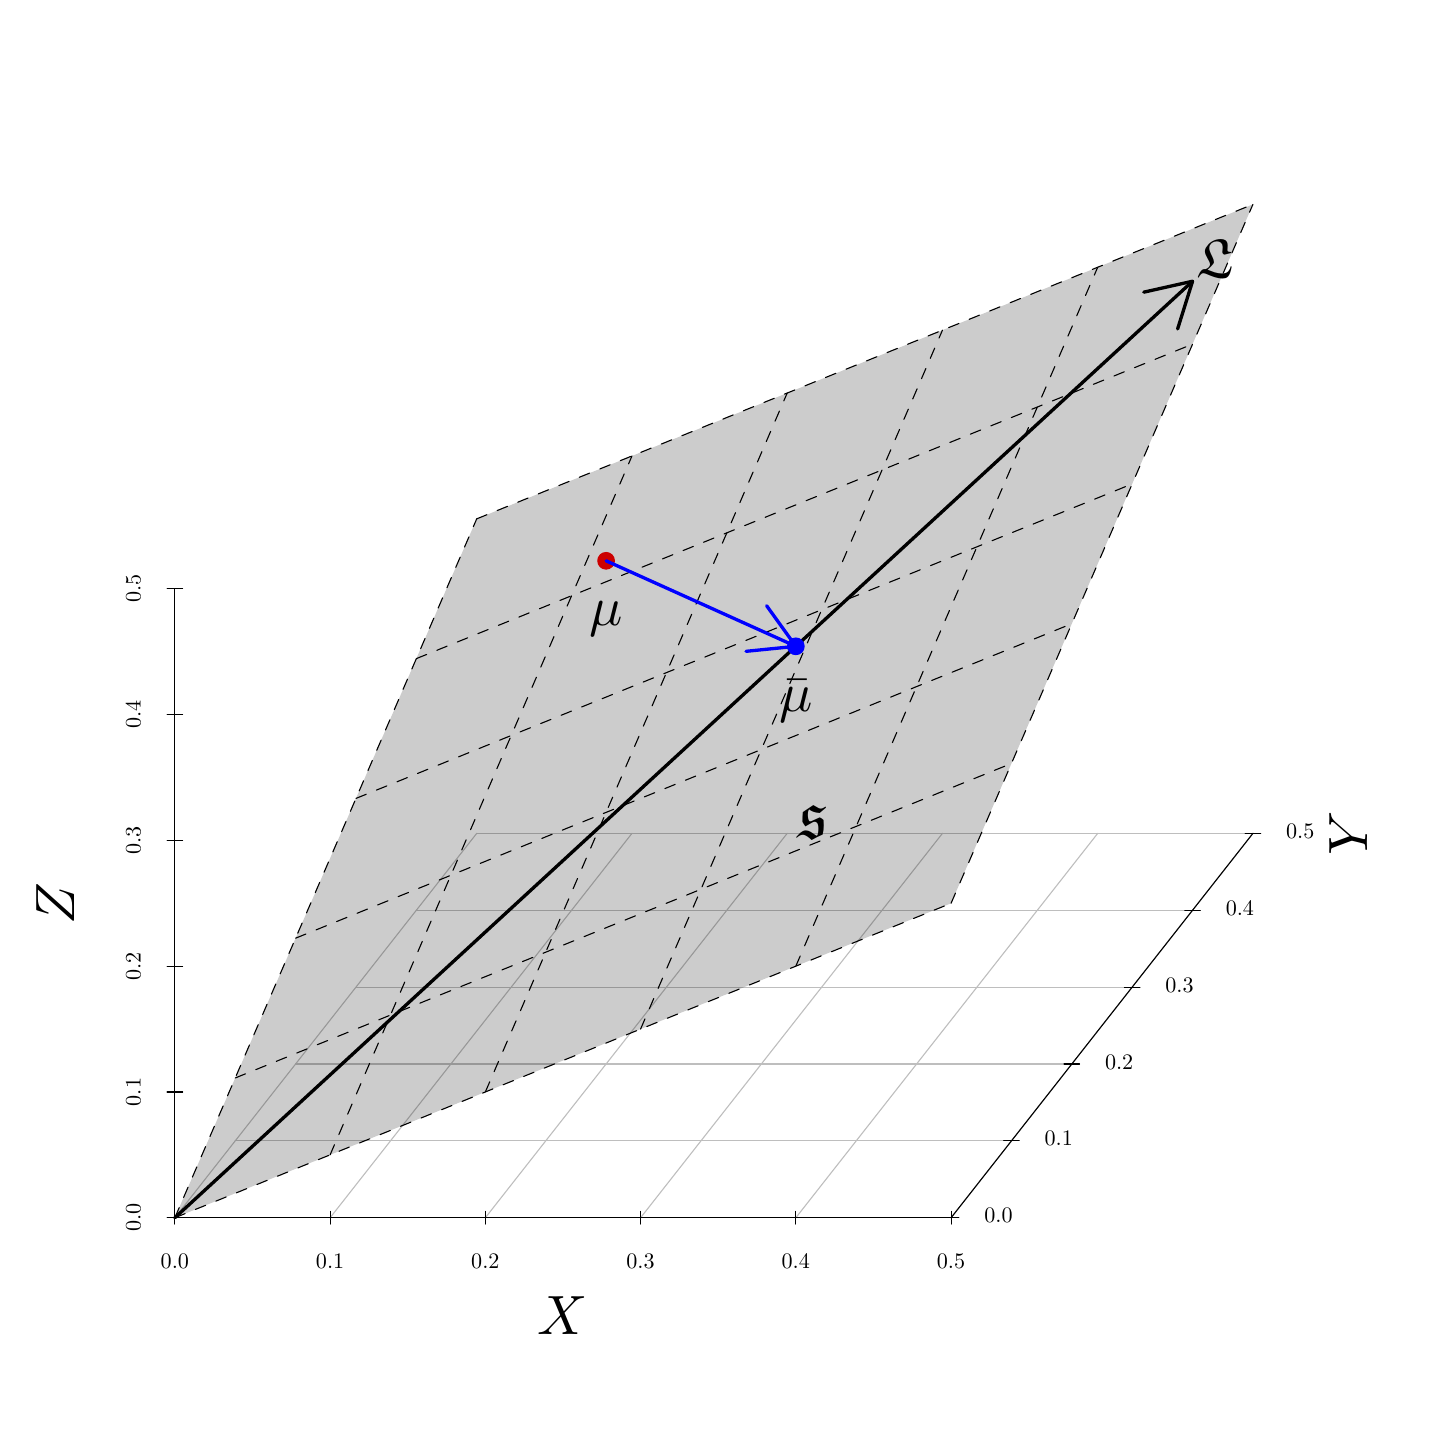
\begin{tikzpicture}[x=1pt,y=1pt]
\definecolor{fillColor}{RGB}{255,255,255}
\path[use as bounding box,fill=fillColor,fill opacity=0.00] (0,0) rectangle (505.89,505.89);
\begin{scope}
\path[clip] ( 37.20, 61.20) rectangle (468.69,456.69);
\definecolor{drawColor}{RGB}{190,190,190}

\path[draw=drawColor,line width= 0.4pt,line join=round,line cap=round] ( 53.18, 75.85) -- (162.26,214.75);

\path[draw=drawColor,line width= 0.4pt,line join=round,line cap=round] (109.28, 75.85) -- (218.36,214.75);

\path[draw=drawColor,line width= 0.4pt,line join=round,line cap=round] (165.38, 75.85) -- (274.45,214.75);

\path[draw=drawColor,line width= 0.4pt,line join=round,line cap=round] (221.47, 75.85) -- (330.55,214.75);

\path[draw=drawColor,line width= 0.4pt,line join=round,line cap=round] (277.57, 75.85) -- (386.65,214.75);

\path[draw=drawColor,line width= 0.4pt,line join=round,line cap=round] (333.67, 75.85) -- (442.74,214.75);

\path[draw=drawColor,line width= 0.4pt,line join=round,line cap=round] ( 53.18, 75.85) -- (333.67, 75.85);

\path[draw=drawColor,line width= 0.4pt,line join=round,line cap=round] ( 75.00,103.63) -- (355.48,103.63);

\path[draw=drawColor,line width= 0.4pt,line join=round,line cap=round] ( 96.81,131.41) -- (377.30,131.41);

\path[draw=drawColor,line width= 0.4pt,line join=round,line cap=round] (118.63,159.19) -- (399.11,159.19);

\path[draw=drawColor,line width= 0.4pt,line join=round,line cap=round] (140.44,186.97) -- (420.93,186.97);

\path[draw=drawColor,line width= 0.4pt,line join=round,line cap=round] (162.26,214.75) -- (442.74,214.75);
\definecolor{drawColor}{RGB}{0,0,0}

\path[draw=drawColor,line width= 0.4pt,line join=round,line cap=round] (330.86, 75.85) -- (336.47, 75.85);

\path[draw=drawColor,line width= 0.4pt,line join=round,line cap=round] (352.68,103.63) -- (358.29,103.63);

\path[draw=drawColor,line width= 0.4pt,line join=round,line cap=round] (374.49,131.41) -- (380.10,131.41);

\path[draw=drawColor,line width= 0.4pt,line join=round,line cap=round] (396.31,159.19) -- (401.92,159.19);

\path[draw=drawColor,line width= 0.4pt,line join=round,line cap=round] (418.12,186.97) -- (423.73,186.97);

\path[draw=drawColor,line width= 0.4pt,line join=round,line cap=round] (439.94,214.75) -- (445.55,214.75);

\path[draw=drawColor,line width= 0.4pt,line join=round,line cap=round] ( 53.18, 73.57) -- ( 53.18, 78.12);

\path[draw=drawColor,line width= 0.4pt,line join=round,line cap=round] (109.28, 73.57) -- (109.28, 78.12);

\path[draw=drawColor,line width= 0.4pt,line join=round,line cap=round] (165.38, 73.57) -- (165.38, 78.12);

\path[draw=drawColor,line width= 0.4pt,line join=round,line cap=round] (221.47, 73.57) -- (221.47, 78.12);

\path[draw=drawColor,line width= 0.4pt,line join=round,line cap=round] (277.57, 73.57) -- (277.57, 78.12);

\path[draw=drawColor,line width= 0.4pt,line join=round,line cap=round] (333.67, 73.57) -- (333.67, 78.12);

\path[draw=drawColor,line width= 0.4pt,line join=round,line cap=round] ( 50.38, 75.85) -- ( 55.99, 75.85);

\path[draw=drawColor,line width= 0.4pt,line join=round,line cap=round] ( 50.38,121.31) -- ( 55.99,121.31);

\path[draw=drawColor,line width= 0.4pt,line join=round,line cap=round] ( 50.38,166.77) -- ( 55.99,166.77);

\path[draw=drawColor,line width= 0.4pt,line join=round,line cap=round] ( 50.38,212.22) -- ( 55.99,212.22);

\path[draw=drawColor,line width= 0.4pt,line join=round,line cap=round] ( 50.38,257.68) -- ( 55.99,257.68);

\path[draw=drawColor,line width= 0.4pt,line join=round,line cap=round] ( 50.38,303.14) -- ( 55.99,303.14);
\end{scope}
\begin{scope}
\path[clip] (  0.00,  0.00) rectangle (505.89,505.89);
\definecolor{drawColor}{RGB}{0,0,0}

\node[text=drawColor,anchor=base,inner sep=0pt, outer sep=0pt, scale=  0.80] at ( 53.18, 57.60) {0.0};

\node[text=drawColor,anchor=base,inner sep=0pt, outer sep=0pt, scale=  0.80] at (109.28, 57.60) {0.1};

\node[text=drawColor,anchor=base,inner sep=0pt, outer sep=0pt, scale=  0.80] at (165.38, 57.60) {0.2};

\node[text=drawColor,anchor=base,inner sep=0pt, outer sep=0pt, scale=  0.80] at (221.47, 57.60) {0.3};

\node[text=drawColor,anchor=base,inner sep=0pt, outer sep=0pt, scale=  0.80] at (277.57, 57.60) {0.4};

\node[text=drawColor,anchor=base,inner sep=0pt, outer sep=0pt, scale=  0.80] at (333.67, 57.60) {0.5};

\node[text=drawColor,rotate= 90.00,anchor=base,inner sep=0pt, outer sep=0pt, scale=  0.80] at ( 40.80, 75.85) {0.0};

\node[text=drawColor,rotate= 90.00,anchor=base,inner sep=0pt, outer sep=0pt, scale=  0.80] at ( 40.80,121.31) {0.1};

\node[text=drawColor,rotate= 90.00,anchor=base,inner sep=0pt, outer sep=0pt, scale=  0.80] at ( 40.80,166.77) {0.2};

\node[text=drawColor,rotate= 90.00,anchor=base,inner sep=0pt, outer sep=0pt, scale=  0.80] at ( 40.80,212.22) {0.3};

\node[text=drawColor,rotate= 90.00,anchor=base,inner sep=0pt, outer sep=0pt, scale=  0.80] at ( 40.80,257.68) {0.4};

\node[text=drawColor,rotate= 90.00,anchor=base,inner sep=0pt, outer sep=0pt, scale=  0.80] at ( 40.80,303.14) {0.5};
\end{scope}
\begin{scope}
\path[clip] ( 37.20, 61.20) rectangle (468.69,456.69);
\definecolor{drawColor}{RGB}{0,0,0}

\node[text=drawColor,anchor=base west,inner sep=0pt, outer sep=0pt, scale=  0.80] at (345.67, 74.01) {0.0};

\node[text=drawColor,anchor=base west,inner sep=0pt, outer sep=0pt, scale=  0.80] at (367.48,101.79) {0.1};

\node[text=drawColor,anchor=base west,inner sep=0pt, outer sep=0pt, scale=  0.80] at (389.30,129.57) {0.2};

\node[text=drawColor,anchor=base west,inner sep=0pt, outer sep=0pt, scale=  0.80] at (411.11,157.35) {0.3};

\node[text=drawColor,anchor=base west,inner sep=0pt, outer sep=0pt, scale=  0.80] at (432.93,185.13) {0.4};

\node[text=drawColor,anchor=base west,inner sep=0pt, outer sep=0pt, scale=  0.80] at (454.74,212.91) {0.5};

\path[draw=drawColor,line width= 0.4pt,line join=round,line cap=round] ( 53.18, 75.85) --
	(333.67, 75.85);
\end{scope}
\begin{scope}
\path[clip] (  0.00,  0.00) rectangle (505.89,505.89);
\definecolor{drawColor}{RGB}{0,0,0}

\node[text=drawColor,anchor=base,inner sep=0pt, outer sep=0pt, scale=  2.00] at (193.42, 33.60) {$X$};
\end{scope}
\begin{scope}
\path[clip] ( 37.20, 61.20) rectangle (468.69,456.69);
\definecolor{drawColor}{RGB}{0,0,0}

\path[draw=drawColor,line width= 0.4pt,line join=round,line cap=round] (333.67, 75.85) --
	(442.74,214.75);
\end{scope}
\begin{scope}
\path[clip] (  0.00,  0.00) rectangle (505.89,505.89);
\definecolor{drawColor}{RGB}{0,0,0}

\node[text=drawColor,rotate= 90.00,anchor=base,inner sep=0pt, outer sep=0pt, scale=  2.00] at (484.29,214.75) {$Y$};
\end{scope}
\begin{scope}
\path[clip] ( 37.20, 61.20) rectangle (468.69,456.69);
\definecolor{drawColor}{RGB}{0,0,0}

\path[draw=drawColor,line width= 0.4pt,line join=round,line cap=round] ( 53.18, 75.85) --
	( 53.18,303.14);
\end{scope}
\begin{scope}
\path[clip] (  0.00,  0.00) rectangle (505.89,505.89);
\definecolor{drawColor}{RGB}{0,0,0}

\node[text=drawColor,rotate= 90.00,anchor=base,inner sep=0pt, outer sep=0pt, scale=  2.00] at ( 16.80,189.49) {$Z$};
\end{scope}
\begin{scope}
\path[clip] ( 37.20, 61.20) rectangle (468.69,456.69);
\definecolor{drawColor}{RGB}{255,0,0}
\definecolor{fillColor}{RGB}{255,0,0}

\path[draw=drawColor,line width= 0.4pt,line join=round,line cap=round,fill=fillColor] (209.01,313.24) circle (  3.00);
\definecolor{fillColor}{RGB}{0,0,0}

\path[fill=fillColor,fill opacity=0.20] ( 53.18, 75.85) --
	(162.26,328.40) --
	(442.74,442.04) --
	(333.67,189.49) --
	cycle;
\definecolor{drawColor}{RGB}{0,0,0}

\path[draw=drawColor,line width= 0.4pt,dash pattern=on 4pt off 4pt ,line join=round,line cap=round] ( 53.18, 75.85) -- (162.26,328.40);

\path[draw=drawColor,line width= 0.4pt,dash pattern=on 4pt off 4pt ,line join=round,line cap=round] (109.28, 98.58) -- (218.36,351.12);

\path[draw=drawColor,line width= 0.4pt,dash pattern=on 4pt off 4pt ,line join=round,line cap=round] (165.38,121.31) -- (274.45,373.85);

\path[draw=drawColor,line width= 0.4pt,dash pattern=on 4pt off 4pt ,line join=round,line cap=round] (221.47,144.04) -- (330.55,396.58);

\path[draw=drawColor,line width= 0.4pt,dash pattern=on 4pt off 4pt ,line join=round,line cap=round] (277.57,166.77) -- (386.65,419.31);

\path[draw=drawColor,line width= 0.4pt,dash pattern=on 4pt off 4pt ,line join=round,line cap=round] (333.67,189.49) -- (442.74,442.04);

\path[draw=drawColor,line width= 0.4pt,dash pattern=on 4pt off 4pt ,line join=round,line cap=round] ( 53.18, 75.85) -- (333.67,189.49);

\path[draw=drawColor,line width= 0.4pt,dash pattern=on 4pt off 4pt ,line join=round,line cap=round] ( 75.00,126.36) -- (355.48,240.00);

\path[draw=drawColor,line width= 0.4pt,dash pattern=on 4pt off 4pt ,line join=round,line cap=round] ( 96.81,176.87) -- (377.30,290.51);

\path[draw=drawColor,line width= 0.4pt,dash pattern=on 4pt off 4pt ,line join=round,line cap=round] (118.63,227.38) -- (399.11,341.02);

\path[draw=drawColor,line width= 0.4pt,dash pattern=on 4pt off 4pt ,line join=round,line cap=round] (140.44,277.89) -- (420.93,391.53);

\path[draw=drawColor,line width= 0.4pt,dash pattern=on 4pt off 4pt ,line join=round,line cap=round] (162.26,328.40) -- (442.74,442.04);

\path[draw=drawColor,line width= 1.2pt,line join=round,line cap=round] ( 53.18, 75.85) -- (420.93,414.26);

\path[draw=drawColor,line width= 1.2pt,line join=round,line cap=round] (415.53,397.02) --
	(420.93,414.26) --
	(403.30,410.31);
\definecolor{drawColor}{RGB}{0,0,255}
\definecolor{fillColor}{RGB}{0,0,255}

\path[draw=drawColor,line width= 0.4pt,line join=round,line cap=round,fill=fillColor] (277.57,282.34) circle (  3.00);

\path[draw=drawColor,line width= 1.2pt,line join=round,line cap=round] (209.01,313.24) -- (277.57,282.34);

\path[draw=drawColor,line width= 1.2pt,line join=round,line cap=round] (259.59,280.53) --
	(277.57,282.34) --
	(267.02,297.00);
\definecolor{drawColor}{RGB}{0,0,0}

\node[text=drawColor,anchor=base west,inner sep=0pt, outer sep=0pt, scale=  2.00] at (422.26,415.64) {{$\mathfrak{L}$}};

\node[text=drawColor,anchor=base,inner sep=0pt, outer sep=0pt, scale=  2.00] at (209.01,289.76) {{$\mu$}};

\node[text=drawColor,anchor=base,inner sep=0pt, outer sep=0pt, scale=  2.00] at (277.57,258.86) {{$\bar{\mu}$}};

\node[text=drawColor,anchor=base west,inner sep=0pt, outer sep=0pt, scale=  1.00] at (278.67,212.91) {{\Huge $\mathfrak{s}$}};
\end{scope}
\end{tikzpicture}

		}
		\caption{$\mathfrak{L}$ is a linear subspace of the coherent subspace $\mathfrak{s}$. If $s\circ g$ is a projection not onto $\mathfrak{s}$ but onto $\mathfrak{L}$, then $\bm{\mu} \in \mathfrak{s}$ will be moved to $\bar{\bm{\mu}} \in \mathfrak{L}$.}\label{fig:Schematic_3D}
	\end{figure}
	
	Finally, it is often stated that an assumption required to prove the unbiasedness preserving property is that $\bm{SGS}=\bm{S}$ or alternatively that $\bm{GS}=\bm{I}$.  Both of these conditions are equivalent to assuming that $\bm{SG}$ is a projection matrix.  \todo{perhaps elaborate in a proof in appendix}  When the problem is viewed through the prism of imposing a constraint $\bm{GS}=\bm{I}$ to ensure unbiasedness is preserved, one may be tempted to deal with biased forecasts by selecting $\bm{G}$ is an unconstrained manner.  However, equipped with a geometric understanding of the problem, we would advise against this approach.  Our own solution to dealing with biased forecasts is discussed in detail in the next section.  
	
	
%	Representation of a coherent subspace in a three dimensional hierarchy where $y_{\text{Tot}} = y_{\text{A}} + y_{\text{B}}$. The coherent subspace is depicted as a gray two dimensional plane labelled $\mathfrak{s}$. Note that the columns of $\vec{s}_1 = (1,1,0)'$ and $\vec{s}_2 = (1, 0, 1)'$ form a basis for $\mathfrak{s}$. The red points lying on $\mathfrak{s}$ can be either realisations or coherent forecasts.
	

	
	
	\section{Bias correction}
	
	\section{Application}
	
	\section{Conclusions}
	
	\newpage
	
	\bibliographystyle{agsm}
	
	\bibliography{References_paper1}
	
\end{document}

